\documentclass[tikz]{standalone}
\usetikzlibrary{calc}
\begin{document}
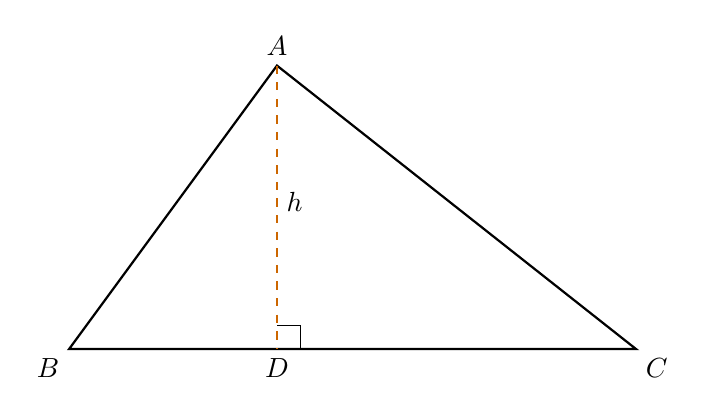
\begin{tikzpicture}[scale=1.2]
  % ---- Segitiga lancip: tinggi dari A ke BC ----
  \begin{scope}
    \coordinate (B) at (0,0);
    \coordinate (C) at (6,0);
    \coordinate (A) at (2.2,3);
    \coordinate (D) at (2.2,0);
    \draw[thick] (B) -- (C) -- (A) -- cycle;
    \draw[dashed, thick, orange!80!black] (A) -- (D);
    \draw ($(D)+(0.25,0)$) -- ($(D)+(0.25,0.25)$) -- ($(D)+(0,0.25)$);
    \node[above right] at ($(A)!0.55!(D)$) {$h$};
    \foreach \p/\pos in {A/above, B/below left, C/below right, D/below}
      \node[\pos] at (\p) {$\p$};
  \end{scope}
\end{tikzpicture}

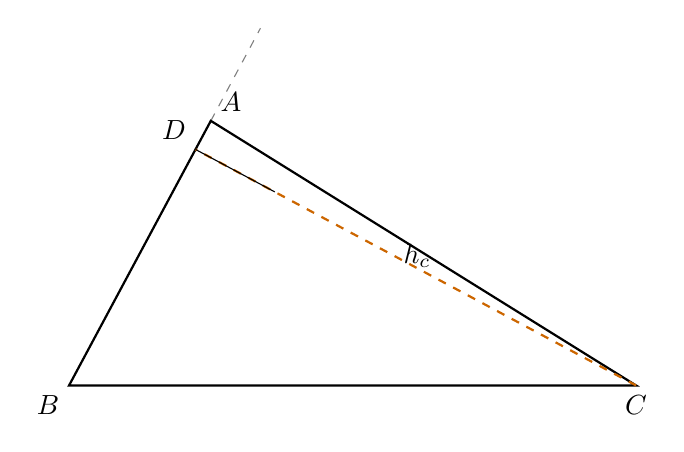
\begin{tikzpicture}[scale=1.2]
  % ---- Segitiga tumpul: tinggi dari C ke perpanjangan AB ----
  % proyeksi C(6,0) ke garis BA: A(1.5,2.8), B(0,0)
  % D = (A.(C-A))/(A.A) * A ; A.A=1.5^2+2.8^2=10.09 ; A.(C-A)=1.5*4.5+2.8*(-2.8)=-1.09
  % hmm -> gunakan proyeksi ke arah dari B: d = ((C-A).(-A))/|A|^2 ... dihitung manual:
  % vektor BA = (1.5,2.8); proyeksi C pada garis: t = C.BA/|BA|^2 = (6*1.5+0)/10.09 = 0.89197
  % D = t*BA = (1.33796, 2.49752) -> titik proyeksi C ke garis AB
  \begin{scope}
    \coordinate (B) at (0,0);
    \coordinate (C) at (6,0);
    \coordinate (A) at (1.5,2.8);
    \coordinate (D) at (1.33796,2.49752);
    \draw[dashed, gray] (A) -- ($(B)!1.35!(A)$);   % perpanjangan BA melewati A
    \draw[thick] (A) -- (B) -- (C) -- cycle;
    \draw[dashed, thick, orange!80!black] (C) -- (D);
    \draw ($(D)!0.18!(C)$) -- ($($(D)!0.18!(C)$)!0.18!(D)+(0,0)$) -- (D);
    \node[right] at ($(C)!0.55!(D)$) {$h_c$};
    \foreach \p/\pos in {A/above right, B/below left, C/below, D/above left}
      \node[\pos] at (\p) {$\p$};
  \end{scope}
\end{tikzpicture}

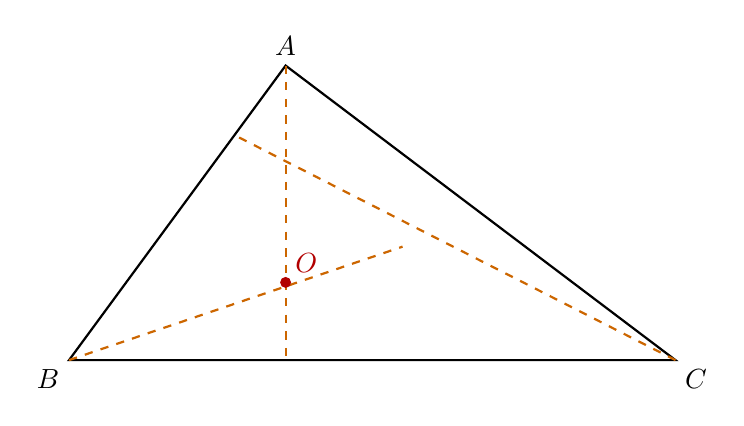
\begin{tikzpicture}[scale=1.1]
  % ---- Tiga tinggi bertemu di ortosenter (segitiga lancip) ----
  \coordinate (B) at (0,0);
  \coordinate (C) at (7,0);
  \coordinate (A) at (2.5,3.4);
  % proyeksi A ke BC
  \coordinate (D1) at (2.5,0);
  % tinggi dari B ke AC
  \coordinate (D2) at (3.85,1.31);
  % tinggi dari C ke AB
  \coordinate (D3) at (1.912,2.596);
  \draw[thick] (B) -- (C) -- (A) -- cycle;
  \draw[dashed, thick, orange!80!black] (A) -- (D1);
  \draw[dashed, thick, orange!80!black] (B) -- (D2);
  \draw[dashed, thick, orange!80!black] (C) -- (D3);
  \fill[red!70!black] (2.5,0.897) circle (1.8pt) node[above right] {$O$};
  \foreach \p/\pos in {A/above, B/below left, C/below right}
    \node[\pos] at (\p) {$\p$};
\end{tikzpicture}
\end{document}
